\def\year{2021}\relax
%File: formatting-instructions-latex-2021.tex
%release 2021.1
\documentclass[letterpaper]{article} % DO NOT CHANGE THIS
\usepackage{aaai21}  % DO NOT CHANGE THIS
\usepackage{times}  % DO NOT CHANGE THIS
\usepackage{helvet} % DO NOT CHANGE THIS
\usepackage{courier}  % DO NOT CHANGE THIS
\usepackage[hyphens]{url}  % DO NOT CHANGE THIS
\usepackage{graphicx} % DO NOT CHANGE THIS

% ADJUSTED BY AFM ----------------------------------------------------------
\usepackage{amsmath} % ENTERED BY AFM
\usepackage{subcaption}
\usepackage[table,usenames,dvipsnames]{xcolor}



\urlstyle{rm} % DO NOT CHANGE THIS
\def\UrlFont{\rm}  % DO NOT CHANGE THIS
\usepackage{natbib}  % DO NOT CHANGE THIS AND DO NOT ADD ANY OPTIONS TO IT
\usepackage{caption} % DO NOT CHANGE THIS AND DO NOT ADD ANY OPTIONS TO IT
\frenchspacing  % DO NOT CHANGE THIS
\setlength{\pdfpagewidth}{8.5in}  % DO NOT CHANGE THIS
\setlength{\pdfpageheight}{11in}  % DO NOT CHANGE THIS
\nocopyright
%PDF Info Is REQUIRED.
% For /Author, add all authors within the parentheses, separated by commas. No accents or commands.
% For /Title, add Title in Mixed Case. No accents or commands. Retain the parentheses.
\pdfinfo{
/Title (ML Assignment 4)
/Author (Anthony Menninger)
/TemplateVersion (2021.1)
} %Leave this
% /Title ()
% Put your actual complete title (no codes, scripts, shortcuts, or LaTeX commands) within the parentheses in mixed case
% Leave the space between \Title and the beginning parenthesis alone
% /Author ()
% Put your actual complete list of authors (no codes, scripts, shortcuts, or LaTeX commands) within the parentheses in mixed case.
% Each author should be only by a comma. If the name contains accents, remove them. If there are any LaTeX commands,
% remove them.

% DISALLOWED PACKAGES
% \usepackage{authblk} -- This package is specifically forbidden
% \usepackage{balance} -- This package is specifically forbidden
% \usepackage{color (if used in text)
% \usepackage{CJK} -- This package is specifically forbidden
% \usepackage{float} -- This package is specifically forbidden
% \usepackage{flushend} -- This package is specifically forbidden
% \usepackage{fontenc} -- This package is specifically forbidden
% \usepackage{fullpage} -- This package is specifically forbidden
% \usepackage{geometry} -- This package is specifically forbidden
% \usepackage{grffile} -- This package is specifically forbidden
% \usepackage{hyperref} -- This package is specifically forbidden
% \usepackage{navigator} -- This package is specifically forbidden
% (or any other package that embeds links such as navigator or hyperref)
% \indentfirst} -- This package is specifically forbidden
% \layout} -- This package is specifically forbidden
% \multicol} -- This package is specifically forbidden
% \nameref} -- This package is specifically forbidden
% \usepackage{savetrees} -- This package is specifically forbidden
% \usepackage{setspace} -- This package is specifically forbidden
% \usepackage{stfloats} -- This package is specifically forbidden
% \usepackage{tabu} -- This package is specifically forbidden
% \usepackage{titlesec} -- This package is specifically forbidden
% \usepackage{tocbibind} -- This package is specifically forbidden
% \usepackage{ulem} -- This package is specifically forbidden
% \usepackage{wrapfig} -- This package is specifically forbidden
% DISALLOWED COMMANDS
% \nocopyright -- Your paper will not be published if you use this command
% \addtolength -- This command may not be used
% \balance -- This command may not be used
% \baselinestretch -- Your paper will not be published if you use this command
% \clearpage -- No page breaks of any kind may be used for the final version of your paper
% \columnsep -- This command may not be used
% \newpage -- No page breaks of any kind may be used for the final version of your paper
% \pagebreak -- No page breaks of any kind may be used for the final version of your paperr
% \pagestyle -- This command may not be used
% \tiny -- This is not an acceptable font size.
% \vspace{- -- No negative value may be used in proximity of a caption, figure, table, section, subsection, subsubsection, or reference
% \vskip{- -- No negative value may be used to alter spacing above or below a caption, figure, table, section, subsection, subsubsection, or reference

\setcounter{secnumdepth}{0} %May be changed to 1 or 2 if section numbers are desired.

% The file aaai21.sty is the style file for AAAI Press
% proceedings, working notes, and technical reports.
%

% Title

% Your title must be in mixed case, not sentence case.
% That means all verbs (including short verbs like be, is, using,and go),
% nouns, adverbs, adjectives should be capitalized, including both words in hyphenated terms, while
% articles, conjunctions, and prepositions are lower case unless they
% directly follow a colon or long dash


%Example, Single Author, ->> remove \iffalse,\fi and place them surrounding AAAI title to use it
\title{
Machine Learning - CS 7641
Assignment 4
	
}
\author {
    % Author
    Anthony Menninger \\
}

\affiliations{
    Georgia Tech OMSCS Program \\
    amenninger3\\
    tmenninger@gatech.edu

}

\begin{document}

\maketitle

\begin{abstract}
This paper explores Markov Decision Processes through the use of Value Iteration, Policy Iteration and Q Learning.  It looks at a simple "Forest" MDP and a larger Frozen Lake "Grid World".
\end{abstract}

\section{Problem Introduction}

A key element in both Markov Decision Processes (MDPs) is the idea of a discount, which is often referred to as \textbf{\emph{Gamma ($\gamma$)}}.  This discount factor, between 1 and 0, allows solutions for infinite MDPs by discounting future value by \textbf{\emph{Gamma}} for each step into the future.  In an infinite activity, this ends up valuing future value at $ \frac{1}{1- \gamma}$.  Gamma close to 0 creates a very close horizon where only immediate rewards are maximized, while Gamma close to 1 creates a long horizon, where maximizing long term reward is emphasized.  As will be seen, MDPs are very sensitive to this and small changes can create very different solutions.

The key toolset I used was the hiive fork [3] of the MDP Toolbox for Python [2], which is derived from the MDP Toolbox [1].  I also used the OpenAI Gym Frozen Lake environment [4] for the larger Frozen Lake MDP.

\subsection{Forest MDP}
\textbf{\emph{Forest MDP}} is a simple MDP from the hiive MDP Toolbox [2] that models the value of a forest with respect to two actions that can be performed each year: \textbf{\emph{wait}} or \textbf{\emph{cut}}.  There is a stochastic element of forest fires that occur with probability \textbf{\emph{p}}.  Each year is a state, with a max of \textbf{\emph{S}} years / states.  Cutting deterministically transitions to the initial state,  \textbf{\emph{state=0}} and provides a \textbf{\emph{cutting reward}} of 0 if in the initial state, \textbf{\emph{cutting reward}} in the final state and a reward of 1 in all other states.  Waiting transitions to the next year, or if in the max state, remains there.  Forest fires provide a stochastic element, with a fire transitioning back to the initial state.  A \textbf{\emph{waiting reward}} only occurs in the max state, \textbf{\emph{state=S}}.  This is a continual MDP, with no terminal or absorbing states. 

The base setup for \textbf{\emph{Forest}} is seven years (\textbf{\emph{S=7}}), a 10\% chance of forest fire (\textbf{\emph{p=0.1}}), a  (\textbf{\emph{cutting reward=2}}) in any state and a (\textbf{\emph{waiting reward = 4}}) only in the final state.

In the context of MDP's, each state has an action that maximizes expected value and the set of maximizing actions for all states is called a \textbf{\emph{policy}}.  This policy can be examined to determine what rational actors are likely going to do. 

There are several very interesting aspects to this problem.  \textbf{\emph{Forest MDP}} models a key choice being made today around ecology and the environment.  What are the rewards needed to keep forests around?  How do maximizing actions (\textbf{\emph{policy}}) change as the chance of forest fires increase?  How does the length of the considered horizon (\textbf{\emph{Gamma discount}}) influence expected outcomes.  

This also highlights a key challenge in MDP's and Reinforcement Learning, which is understanding rewards and setting them appropriately.  \textbf{\emph{Forest MDP}}  allows modeling of different situations to inform the construction of public policy for governments, NGO's and corporations.  The \textbf{\emph{cutting reward}} might be clearly modeled using expected timber value, but other types of reward may want to be considered in the \textbf{\emph{waiting reward}}, such as carbon reduction and maintenance of ecological diversity.  This MDP can be used to model economic rewards and penalties to compel desired outcomes, such as a carbon tax that would reduce the value of the \textbf{\emph{cutting reward}}.

As described, this MDP is more likely to be "solved" using Value Iteration (VI) or Policy Iteration (PI) in order to use it for comparing different tradeoffs and outcomes.

\subsection{Lake MDP}
\textbf{\emph{Lake MDP}} is a larger MDP that uses the OpenAI gym Frozen Lake [4,5] to create its environment.   It is a 2D grid with four actions to move \textbf{\emph{up, down, left, right}} and can be of \textbf{\emph{Size}}, which is the number of grids on one size of the square, creating \textbf{\emph{Size x Size}} states.  The lake can be set to not slippery, where the action is deterministic, or slippery, where the action is stochastic.  When slippery, the action has a 1/3 chance of moving in the desired direction, a 1/3 to the left of the desired direction and 1/3 to the right of the desired direction, which is fairly stochastic.  This is an episodic MDP where the player starts in the first state - (0,0) upper left corner.  The goal state (size, size) is in the bottom right corner and has a reward of 1.  There are also random holes which are absorbing states with a reward of 0.

I created Small (\textbf{\emph{Size=4}}), Medium (\textbf{\emph{Size=8}}), and Large (\textbf{\emph{Size=16}}) worlds to explore the impacts of different size worlds.  

This MDP is interesting because it embodies a core Reinforcement Learning challenge of exploring an environment and learning what to do.  It describes a common, everyday task of exploring an environment and learning where the rewards and traps are.  Robots are often in a situation where they need to move about and find out what they should be doing.  In addition, it creates a much more interesting set of transitions between the different states, as compared with the \textbf{\emph{Forest MDP}}, where transitions are either next state or back to beginning.  Also, \textbf{\emph{Lake MDP}} is episodic vs  \textbf{\emph{Forest MDP}} which is continual.

As described, this MDP is more likely to be "learned" in a setting using Q Learning to explore how agents use reinforcement learning to learn to navigate and behave in an unknown environment.

\section{Forest MDP Value Iteration (VI) and Policy Iteration (PI)}
We start with the \textbf{\emph{Forest MDP}}.   The VI and PI implementations used for this experiment started with the hiive MDP Toolbox [3], which was then "forked" to allow for modifications for this analysis.  Both VI and PI are model based algorithms, which means that the complete MDP is known and used for solving the problem.  This matches the \textbf{\emph{Forest MDP}} because it likely to be used to model different situations to see the impacts of different parameters.   

Both VI an PI rely on the Bellman Equation, which can be represented in different ways as seen in  \textbf{Equation \ref{eq:bellman}} 
\begin{equation} 
\label{eq:bellman}
V(s) = R(s) + \gamma \; max_{a^\prime}  \sum_{s^\prime} T(s,a,s^\prime) V(s^\prime)
\end{equation}

With Value Iteration, a sweep is performed of all states to update the Values using \textbf{Equation \ref{eq:bellman}}.  If this is run to infinity, it will converge to the exact solution.  Practically, a setting of acceptable error is created to determine convergence, with each iteration comparing the old values and new values to determine error.  I will refer to this error threshold as the \emph{E Stop} value.  In some discussions it is also confusingly referred to as $\epsilon$,  which is the same designation for exploration in Q Learning. 

\textbf{Figure \ref{fig:forest_vi}} shows the VI solution for the default setup of the  \textbf{\emph{Lake MDP}} outlined in the introduction with the default VI setting of \emph{Error Threshold=0.01}.  First, we can see that it takes 49 iterations to solve.  Initially, the values for all states are low, but over time the values increase and shift from the high value end state towards the initial state.  As the values increase, the policy changes from cutting in almost all states to waiting in all states.  The final policy is reached in 7 iterations, but the final emph{Error Threshold} values aren't reached for much later.  Looking at the value of the final state, even though we only get a reward of 4 for waiting, our expected value in that state is almost 27 because with this policy we will stay there until a forest fire forces a transition. 

\begin{figure}[!htb]
\centering
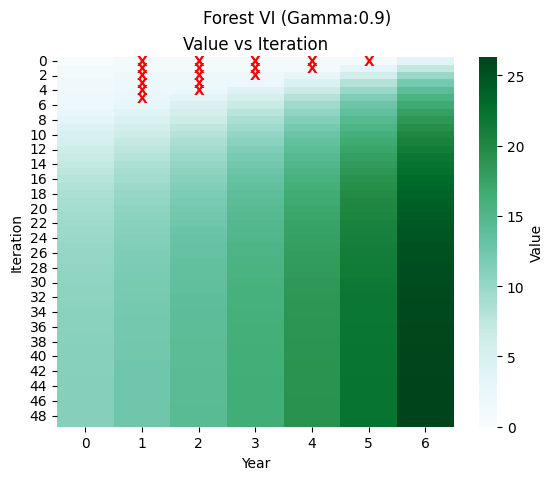
\includegraphics[width=2.75in, height=2.75in]{Figures/Forest_VI_Gamma_0_9_Value_vs_Iteration.png}
\caption{Forest MDP Value Iteration (VI) with \emph{Error Threshold=0.01}. Red X indicates the cut action, otherwise the action is wait. }
\label{fig:forest_vi}
\end{figure}


\begin{figure}[!htb]
 	\begin{subfigure}[b]{0.45\textwidth}
	\centering
		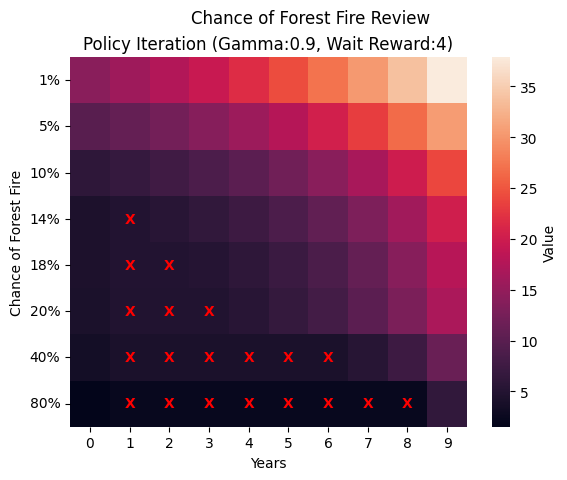
\includegraphics[width=2.75in]{Figures/Chance_of_Forest_Fire_Review_Policy_Iteration_Gamma_0_9__Wait_Reward_4.png}
		\caption{Discount of 0.9 and a wait reward of 4. }
  	\end{subfigure}
	\centering
	 \begin{subfigure}[b]{0.235\textwidth}
		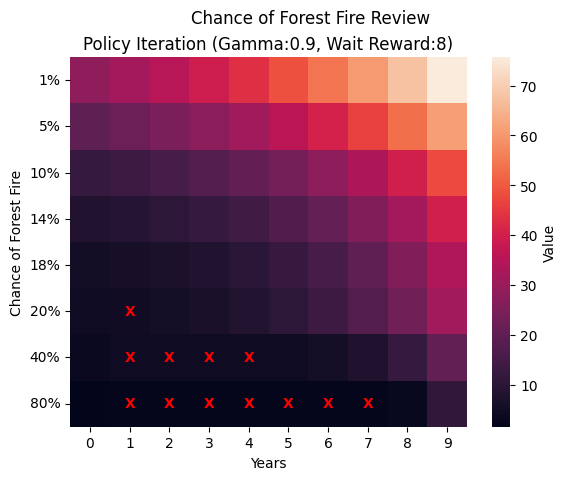
\includegraphics[width=1.7in]{Figures/Chance_of_Forest_Fire_Review_Policy_Iteration_Gamma_0_9__Wait_Reward_8.png}
		\caption{A wait reward of 8. }
  	\end{subfigure}%
	\begin{subfigure}[b]{0.235\textwidth}
		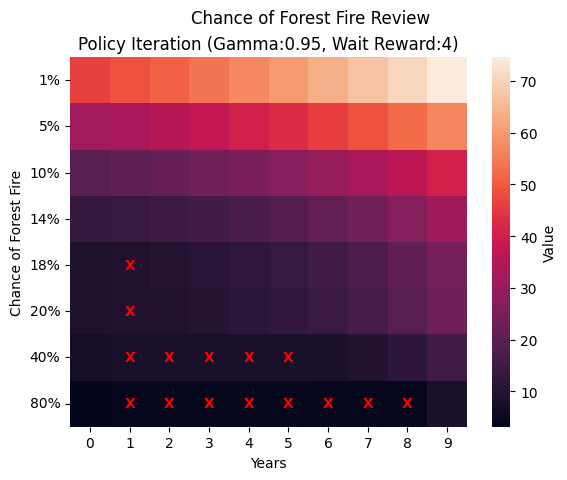
\includegraphics[width=1.7in]{Figures/Chance_of_Forest_Fire_Review_Policy_Iteration_Gamma_0_95__Wait_Reward_4.png}
		\caption{Discount of 0.95}
  	\end{subfigure}
\caption{Forest Values and Policy vs Chance of Forest Fire for a 10 year MDP}
\label{fig:forest_fire_base}
\end{figure}

An important concern today is the increase in forest fires due to climate change.  \textbf{Figure \ref{fig:forest_fire_base} a} shows how increases in the chance of forest fires dramatically reduces the values associated with waiting and optimal policies more likely to increase cutting.  One way to reduce cutting is to increase the reward to wait.   \textbf{Figure \ref{fig:forest_fire_base} b} shows this, with the reward increased to 8.  We can see that cutting has been reduced vs the base, as well as dramatically increasing the values associated with states.  We can also increase the horizon of our valuation by increasing Gamma, the discount factor.  Increasing Gamma to 0.95 from 0.9, in \textbf{Figure \ref{fig:forest_fire_base} c}, also dramatically increases the value and reduces cutting.  This demonstrates the power of an MDP to explore different parameters to model outcomes and inform decision making.


\begin{figure}[!htb]
\centering
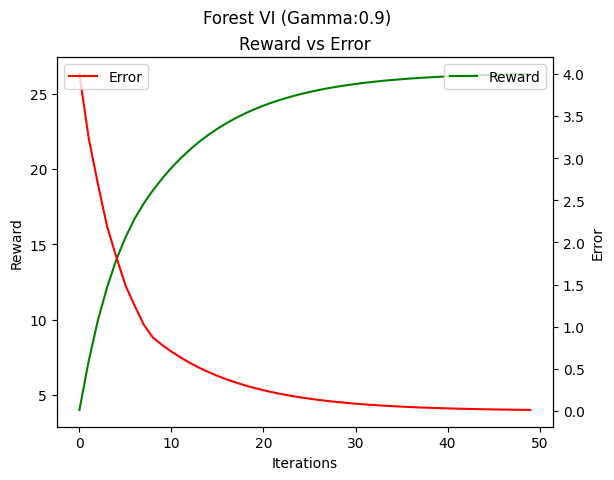
\includegraphics[width=2.75in, height=2.75in]{Figures/Forest_VI_Gamma_0_9_Reward_vs_Error.png}
\caption{Forest MDP Value Iteration (VI) Error and Reward vs Iterations}
\label{fig:forest_vi_reward_error}
\end{figure}
From a technical standpoint, we are often interested in how quickly and accurately an algorithm performs. \textbf{Figure \ref{fig:forest_vi_reward_error}} shows the Reward and Error per iteration of VI, with smoothly increasing value and decreasing error.  Error is the maximum difference between an iterations values and the previous iterations values for each state.


\begin{figure}[!htb]
	\begin{subfigure}[b]{0.25\textwidth}
	\centering
		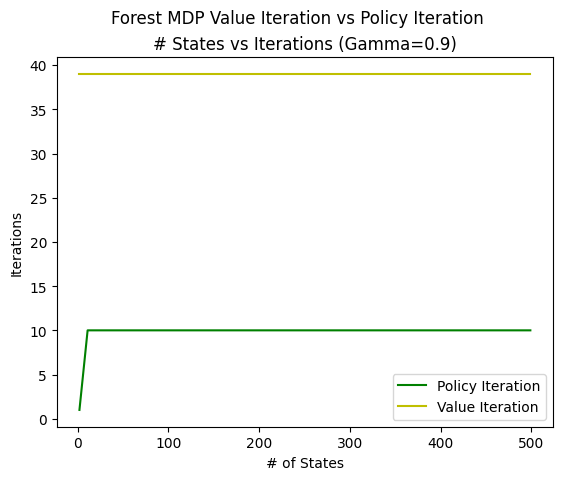
\includegraphics[width=1.75in]{Figures/Forest_MDP_Value_Iteration_vs_Policy_Iteration_num_States_vs_Iterations_Gamma_0_9.png}
		\caption{Iterations vs \# of States}
  	\end{subfigure}%
	\begin{subfigure}[b]{0.25\textwidth}
	\centering
		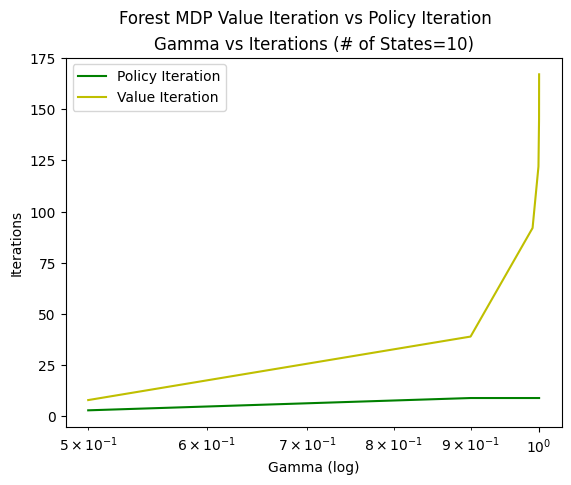
\includegraphics[width=1.75in]{Figures/Forest_MDP_Value_Iteration_vs_Policy_Iteration_Gamma_vs_Iterations_num_of_States_10.png}
		\caption{Iterations vs Gamma Values}
  	\end{subfigure}%
\caption{Forest MDP Iterations till Convergence}
\label{fig:forest_states_vs_iterations}
\end{figure}

An important question is what impacts how many iterations it takes to converge?  \textbf{Figure \ref{fig:forest_states_vs_iterations} a} shows the number of iterations needed to solve the MDP as a function of the number of states.  When I first saw this, I thought it must be wrong!  The number of states in the MDP does not impact the number of iterations to solve for both VI and PI.  This triggered a lot of review and it turns out that the VI algorithm is using a very specific way to determine convergence.  

\begin{equation} 
\label{eq:vi_convergence}
\begin{gathered}
K = \left[ \frac{ log \left[ \frac{2R_{max} }{\epsilon (1 - \gamma)}\right] } {log(\frac{1} {gamma})}\right]\\
if || V - V^* || < \epsilon \;\; then \;\; ||V^{\pi^i} - V^*||_\infty < 2 \epsilon \frac{\gamma}{(1 - \gamma)}
\end{gathered}
\end{equation}

 The top of \textbf{Equation \ref{eq:vi_convergence}} shows how the number of iterations, K, can be solved for depending on the maximum reward, the error $\epsilon$ (not exploration yet) and the discount factor. It does not include any reference to state!  The bottom part can be solved along with K to determine the number of iterations to produce a policy that is $\epsilon$ accurate, which is the effective convergence in the MDP VI algorithm.  
 
\textbf{Figure \ref{fig:forest_states_vs_iterations} b} shows VI's sensitivity to $gamma$, with increasing values requiring more iterations to solve.  Intuitively this makes sense with larger $gamma$ having a longer horizon, requiring many passes to reach the long term value.  The amount of time needed for increasing $gamma$ closely follows this chart and is not reproduced. 


\begin{figure}[!htb]
\centering
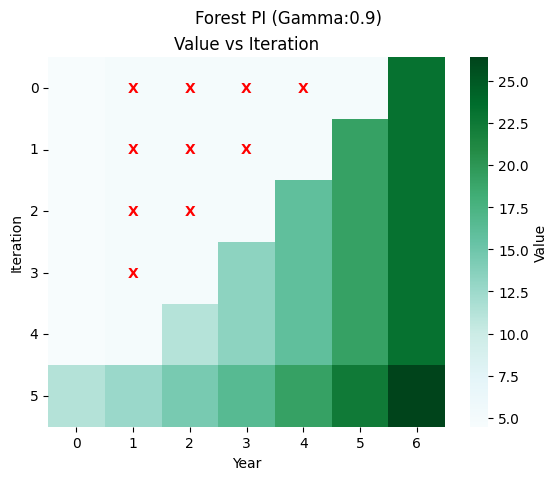
\includegraphics[width=2.75in, height=2.75in]{Figures/Forest_PI_Gamma_0_9_Value_vs_Iteration.png}
\caption{Forest MDP Policy Iteration (PI). Red X indicates the cut action, otherwise the action is wait. }
\label{fig:forest_pi}
\end{figure}

\begin{figure}[!htb]
\centering
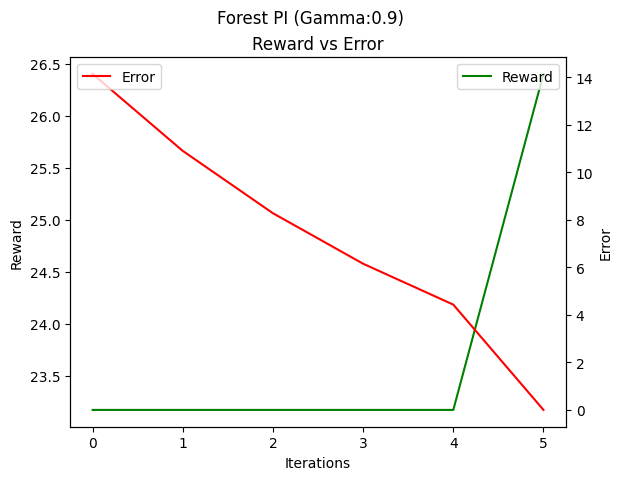
\includegraphics[width=2.75in, height=2.75in]{Figures/Forest_PI_Gamma_0_9_Reward_vs_Error.png}
\caption{Forest MDP Policy Iteration (PI) Error and Reward vs Iterations}
\label{fig:forest_pi_reward_error}
\end{figure}

Policy Iteration (PI) usually requires many fewer iterations than VI.  PI's \textbf{Figure \ref{fig:forest_pi}} shows this, with it converging in 5 iterations, which is many fewer than VI.   \textbf{Figure \ref{fig:forest_pi_reward_error}} shows the reward and error curves per iteration, which are not smooth.  

\begin{equation} \label{eq:value_policy}
\begin{gathered}
Value(s) = max_a Q(s,a)\\
Policy(s) = argmax_a Q(s,a)
\end{gathered}
\end{equation}

PI starts with an initial settings, in this case with all state values set to 0.  It then solves for the policy using a linear solver and the initial Values.  With this new policy, it then recalculates all V values using the Bellman Equation \textbf{\ref{eq:bellman}}.  This implementation of PI uses the Q update rule in \textbf{Equation \ref{q_bellman}}, and then derives the policy and values from that as seen in  \textbf{Equations \ref{eq:value_policy}}.  It is considered converged when the error is 0.  We will see in the \textbf{\emph{Lake MDP}} section that this can be problematic.  In most cases, it exactly solves the MDP, while VI only approximates it to some tolerance.  VI and PI produced the same policies, but there were small Value differences, with these differences almost two orders of magnitude below the correct PI values.

\begin{figure}[!htb]
\centering
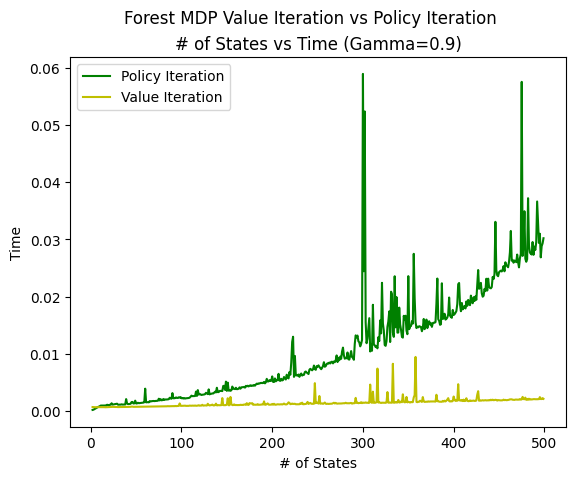
\includegraphics[width=2.75in, height=2.75in]{Figures/Forest_MDP_Value_Iteration_vs_Policy_Iteration_num_of_States_vs_Time_Gamma_0_9.png}
\caption{Forest MDP Time to Solve vs Number of States}
\label{fig:forest_vi_pi_time}
\end{figure}

As seen in \textbf{Figure \ref{fig:forest_states_vs_iterations}}, PI requires fewer iterations to converge than VI and the number of states does not impact the number of iterations needed.  It also is only slightly impacted by increasing Gamma ($\gamma$), while VI was strongly impacted.  It looks like a clear winner.  However,  \textbf{Figure \ref{fig:forest_vi_pi_time}} shows the challenge with PI.  Even though it takes fewer iterations, solving the linear equations is time consuming and very sensitive to the number of states.

\section{Lake MDP Value Iteration (VI) and Policy Iteration (PI)}


\begin{figure*}[!htb]
\centering
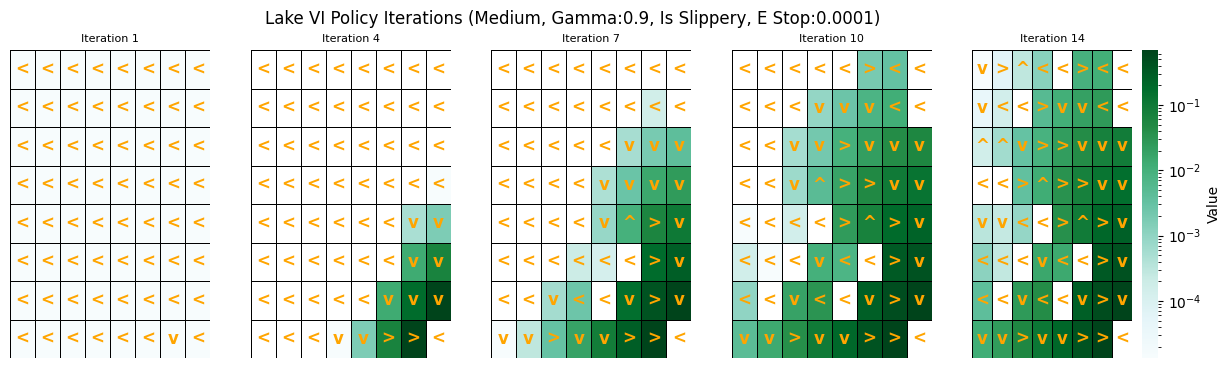
\includegraphics[width=7in]{Figures/Lake_VI_Policy_Iterations_Medium__Gamma_0_9__Is_Slippery__E_Stop_0_0001_Iter_0_to_13_.png}
\caption{Lake MDP Value Iteration}
\label{fig:lake_vi}
\end{figure*}

\textbf{Figure \ref{fig:lake_vi}} shows the \textbf{\emph{Lake MDP}} for the Medium Map.  This is a little clearer than the Large map for highlighting key elements.  Like with the Forest, we can see as that with iterations, value spreads from its sources, in this case the Goal state in the bottom right corner.  As the value spreads, the arrows which indicate the policies action direction change.  The empty value spots are holes, with value 0 and policy directions point away from them where possible.  


\begin{figure}[!htb]
\centering
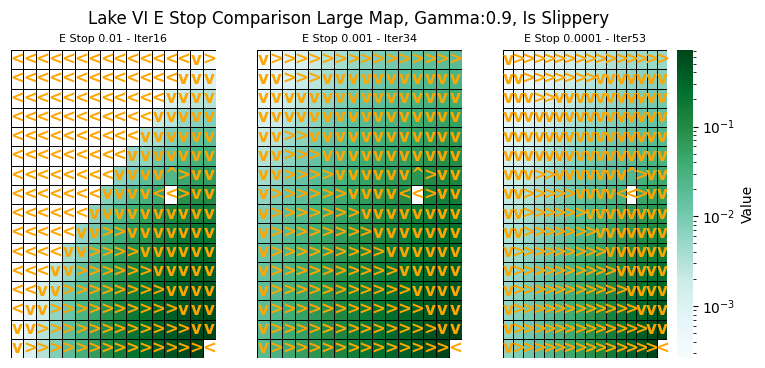
\includegraphics[width=2.75in]{Figures/Lake_VI_E_Stop_Comparison_Large_Map__Gamma_0_9__Is_Slippery_gamma_0_01_to_0_0001_.png}
\caption{Lake MDP Different E Stop \ $\epsilon$ values}
\label{fig:lake_vi_estop}
\end{figure}

A key thing to note is the E Stop ($\epsilon$) value.  When I initially compared the results of the VI vs PI for the \textbf{\emph{Lake MDP}}, I found a significant number of differences in value and policy.  After digging in, I realized that the maximum value of this MDP was around .7.  The E Stop value is an absolute number and the default of 0.01 was much higher than the expected outcomes close the start state, which accounted for the differences.  By decreasing E Stop ($\epsilon$), it allowed for more accurate convergence, seen in \textbf{Figure \ref{fig:lake_vi_estop}}, creating only small value differences between VI and PI.  Once again, small differences in parameters produce very different outcomes.  

\begin{figure}[!htb]
	\begin{subfigure}[b]{0.25\textwidth}
	\centering
		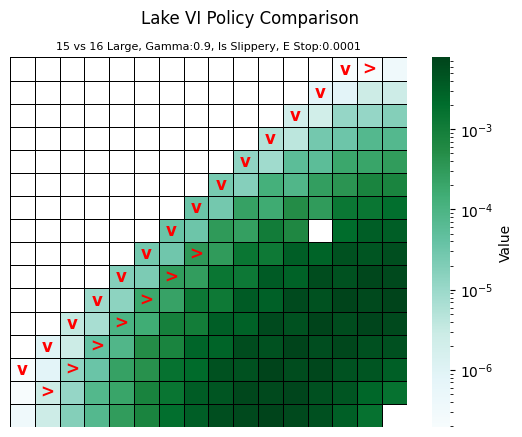
\includegraphics[width=1.75in]{Figures/Lake_VI_Policy_Comparison_15_vs_16_Large__Gamma_0_9__Is_Slippery__E_Stop_0_0001.png}
		\caption{Value Iteration}
  	\end{subfigure}%
	\begin{subfigure}[b]{0.25\textwidth}
	\centering
		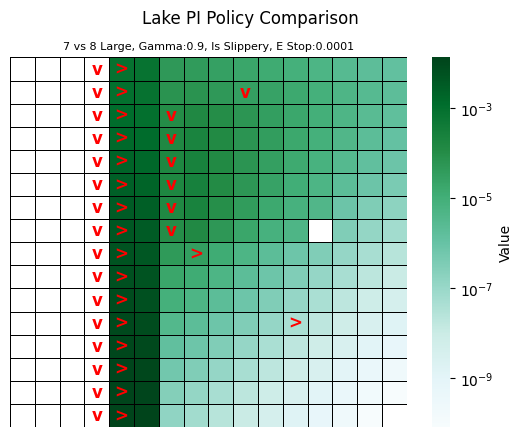
\includegraphics[width=1.75in]{Figures/Lake_PI_Policy_Comparison_7_vs_8_Large__Gamma_0_9__Is_Slippery__E_Stop_0_0001.png}
		\caption{Policy Iteration}
  	\end{subfigure}%
\caption{Lake MDP Comparing Iterations.  Red Arrows indicate where policy changes and the green highlights how much the value has changed.}
\label{fig:lake_iteration_comparison}
\end{figure}

\begin{figure}[!htb]
\centering
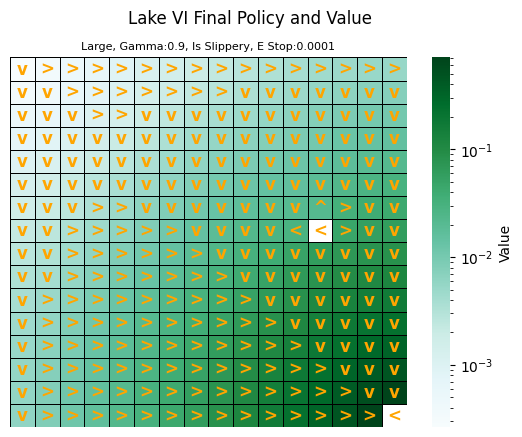
\includegraphics[width=2.75in]{Figures/Lake_VI_Final_Policy_and_Value_Large__Gamma_0_9__Is_Slippery__E_Stop_0_0001.png}
\caption{Large Lake PI solution}
\label{fig:lake_pi_large_solution}
\end{figure}

\textbf{Figure \ref{fig:lake_iteration_comparison} a} is another take on how VI works, comparing Iteration 15 to 16 and highlighting the Value and Policy differences.  The value changes slowly as it spreads from the reward state, changing policy along its change edge, but as it continues to change, we can see a second wave of policy changes.  This is in contrast to PI in \textbf{b}, which moves dramatically with each iteration.  \textbf{Figure \ref{fig:lake_pi_large_solution}} shows the Large Lake PI solution, which would be the most accurate.

\begin{figure}[!htb]
\centering
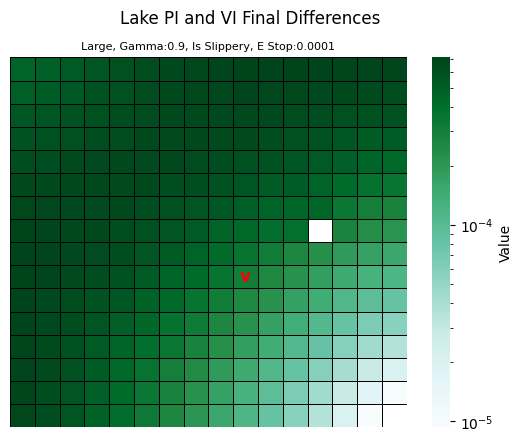
\includegraphics[width=2.75in]{Figures/Lake_PI_and_VI_Final_Differences_Large__Gamma_0_9__Is_Slippery__E_Stop_0_0001.png}
\caption{Large Lake Differences between VI and PI solutions}
\label{fig:lake_vi_pi_difference}
\end{figure}

\textbf{Figure \ref{fig:lake_vi_pi_difference}} shows the difference on the large map between the VI and PI solutions.  The value scale shows that the differences are small, but increase farther away from the source of the reward, as well as one policy difference.  These differences could be reduced further by lowering E Stop ($\epsilon$), but would require more iterations for VI.

\begin{figure}[!htb]
	\begin{subfigure}[b]{0.25\textwidth}
		\centering
		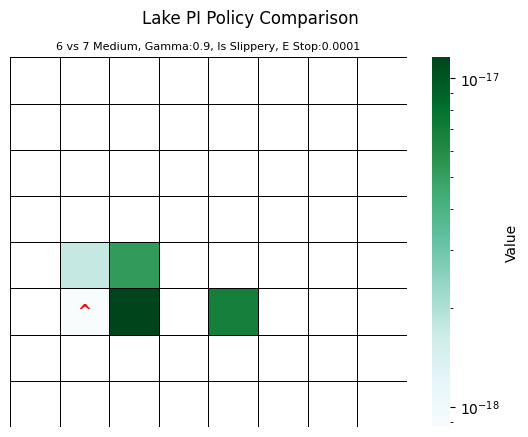
\includegraphics[width=1.75in]{Figures/Lake_PI_Policy_Comparison_6_vs_7_Medium__Gamma_0_9__Is_Slippery__E_Stop_0_0001.png}
  	\end{subfigure}%
	\begin{subfigure}[b]{0.25\textwidth}
		\centering
		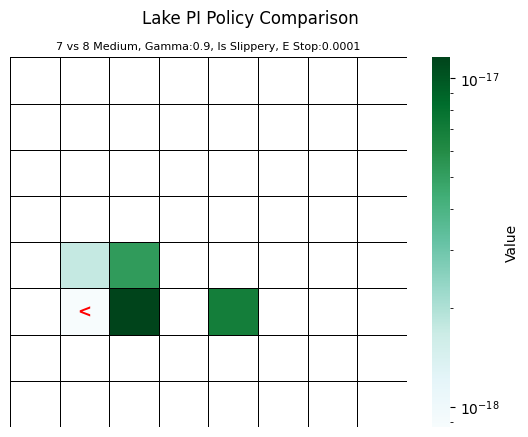
\includegraphics[width=1.75in]{Figures/Lake_PI_Policy_Comparison_7_vs_8_Medium__Gamma_0_9__Is_Slippery__E_Stop_0_0001.png}
  	\end{subfigure}%
\caption{Lake MDP Policy Iteration Oscillating Non Convergence}
\label{fig:lake_pi_oscillation}
\end{figure}

One interesting thing was found regarding convergence for PI on the Medium Lake Map.  When looking at number of iterations, it would use up to the maximum number of iterations (100), essentially not converging.  \textbf{Figure \ref{fig:lake_pi_oscillation}} shows what was happening.  The linear solver was solving very slightly different values, bouncing back and forth between two states, never reaching an error of 0.  Notice the extremely small scale of change - $10^{-17}$, which is a product of floating point math.  A check could be added to this algorithm that the error doesn't need to be zero, but below some extreme amount, like $10^{-15}$.

The VI and PI error and reward curves for  the \textbf{\emph{Lake MDP}} were similar in form to the \textbf{\emph{Forest MDP}} and not reproduced in the paper.

\section{Q Learning}
VI and PI are model based algorithms which use the fully defined model for solving.  This is not practical in many situations in the real world, where we are exploring an environment.  Q Learning is a model free algorithm, which will learn a policy by interacting with an environment.  This uses the Q form of the Bellman Equation, shown in \textbf{Equation \ref{eq:q_learning}}.  One of the first key differences is that instead of sweeping all states in each iteration, now each iteration is one state, action, reward, next state step.  We can expect more, shorter iterations.   While \textbf{\emph{Forest MDP}} is continual, we will also review episodes as another key concept in the \textbf{\emph{Lake MDP}} section.

\begin{equation} 
\label{eq:q_learning}
\hat{Q}(s,a) \xleftarrow{\alpha_t} R(s) + \gamma \;  max_{a^\prime} Q(s^\prime, a^\prime)
\end{equation}

The next key concept is that of exploration vs exploitation. There is a tension between maximizing reward using what is know versus accepting a lower immediate reward in order to find better new rewards.  A common model is to explore with chance $\epsilon$ or maximize with chance (1-$\epsilon$).  This is called an \textbf{$\epsilon$ Greedy} policy.  By lowering $\epsilon$ over time by some decay factor, an environment can be explored and then gradually maximized.  The decay used by the MDP algorithm is geometric, which decays by a certain percentage each step, subject to a minimum floor.

After reviewing the Q Learning MDP algorithm, I realized that there was a randomizing step that every 100 iterations would restart in a random state. These random restarts significantly sped up exploration. I decided to remove this in my forked version because I thought it was "cheating".  When considering an exploration environment, it seemed like a cop-out to magically teleport to any space, cutting out the often difficult exploration to find maximum reward.  

The final key concept is that of the learning factor, \textbf{$\alpha$}, which governs by how much Q is updated on each step. This also decayed over time to take big steps to learn quickly initially, but then taking much smaller steps to not be thrown around by stochastic actions or rewards. 

We will see that Q learning requires substantially tuning of hyper parameters to get a good solution.  In addition, we will explore convergence conditions using running reward and Error.

\subsection{Forest MDP} 

\begin{figure}[!htb]
\centering
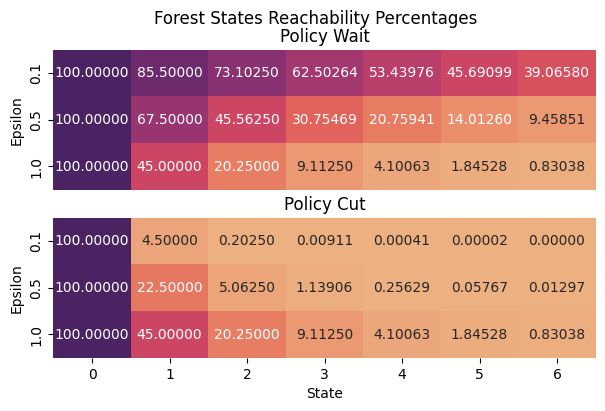
\includegraphics[width=2.75in]{Figures/Forest_States_Reachability_Percentages.png}
\caption{Forest MDP Exploration Reachability Percentages for Q Learning}
\label{fig:forest_q_reachability}
\end{figure}
The first challenge with the \textbf{\emph{Forest MDP}} is that the maximum reward state is the far from the starting state at the end of a set of stochastic transitions.   \textbf{Figure \ref{fig:forest_q_reachability}} shows the percentage chance of reaching each state for a given policy and $\epsilon$.  At the start of Q Learning, $\epsilon$ is 1 to explore.  Here we see that we have less than a 1\% chance of reaching the final state.  What this means is that it will take a lot of iterations to eventually get information about the end state.  In addition, until the end state is observed, policy will lean towards cutting, as that provides a reward.  

\begin{figure}[!htb]
	\begin{subfigure}[b]{0.25\textwidth}
		\centering
		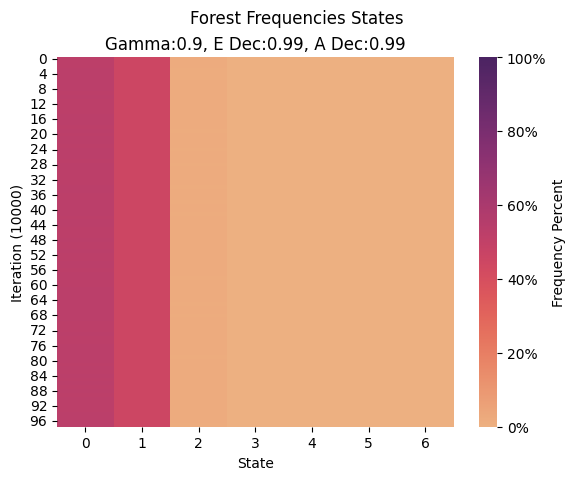
\includegraphics[width=1.75in]{Figures/Forest_Frequencies_States_Gamma_0_9__E_Dec_0_99__A_Dec_0_99.png}
  	\end{subfigure}%
	\begin{subfigure}[b]{0.25\textwidth}
		\centering
		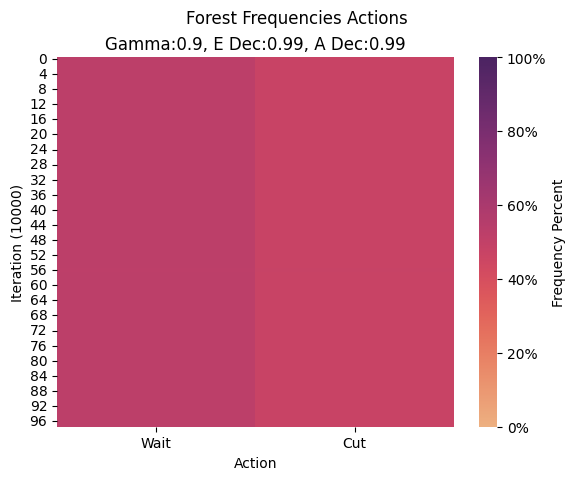
\includegraphics[width=1.75in]{Figures/Forest_Frequencies_Actions_Gamma_0_9__E_Dec_0_99__A_Dec_0_99.png}
  	\end{subfigure}%
\caption{Forest Q,  $\epsilon$ Decay of .99, $\alpha$ Decay of 0.99}
\label{fig:forest_q_e_99_a_99_frequencies}
\end{figure}

\textbf{Figure \ref{fig:forest_q_e_99_a_99_frequencies}} shows the frequencies of actions and of visiting states at different iteration points.  The iteration scale is in 10,000 increments, which shows that an increase in the number of iterations of 5 orders of magnitude versus VI and PI. Ouch!  The left chart shows state frequency, which shows that all time is spent in states 0 and 1.  The right shows that the actions are almost evenly split between cut and wait.  The policy learned was to wait in state 0, cut in state 1.

\begin{figure}[!htb]
	\centering
 	\begin{subfigure}[b]{0.175\textwidth}
		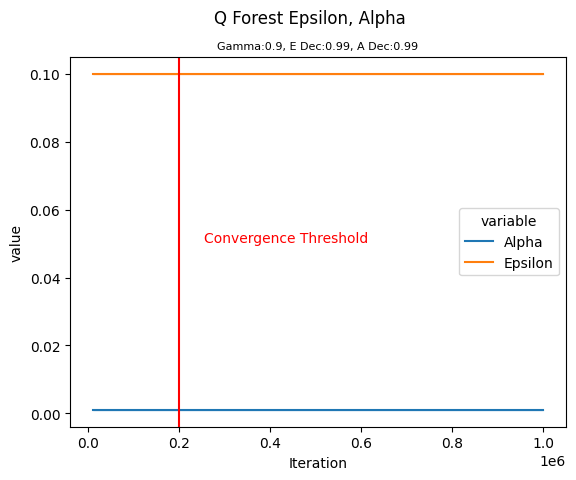
\includegraphics[width=1.2in]{Figures/Q_Forest_Epsilon__Alpha_Gamma_0_9__E_Dec_0_99__A_Dec_0_99.png}
  	\end{subfigure}%
	 \begin{subfigure}[b]{0.175\textwidth}
		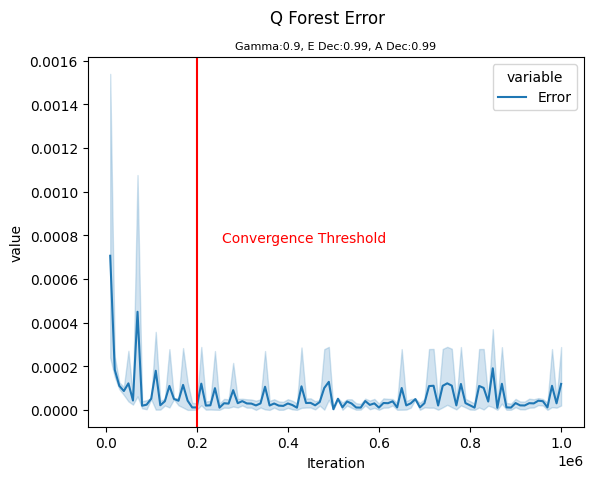
\includegraphics[width=1.2in]{Figures/Q_Forest_Error_Gamma_0_9__E_Dec_0_99__A_Dec_0_99.png}
  	\end{subfigure}%
	\begin{subfigure}[b]{0.175\textwidth}
		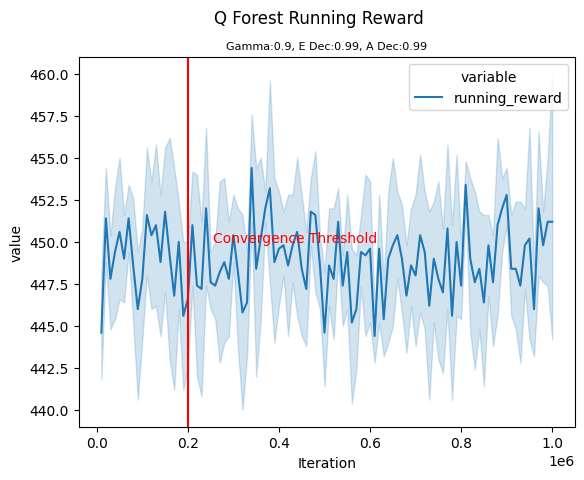
\includegraphics[width=1.2in]{Figures/Q_Forest_Running_Reward_Gamma_0_9__E_Dec_0_99__A_Dec_0_99.png}
  	\end{subfigure}
\caption{Forest Q,  $\epsilon$ Decay of .99, $\alpha$ Decay of 0.99}
\label{fig:forest_q_e_99_a_99_rewards}
\end{figure}

\textbf{Figure \ref{fig:forest_q_e_99_a_99_rewards}} provides insight.  The left chart shows $\epsilon$ and $\alpha$ low and unchanged.  A decay of 0.99 declines to its floor quickly.  The middle chart shows the error at each given iteration.  First, it is very low, which makes sense because only one state is changing per iteration.  It is quite noisy, but does have a declining initial pattern.  The right chart  takes the cumulative reward over the last 1000 iterations at each point.  This is the most important chart and shows how we are doing and the initial settings made all progress in the first few iterations, which don't show on this chart.  I will describe the convergence threshold line in reviewing \textbf{Figure \ref{fig:forest_q_e_99999_a_99999_rewards}}.

\begin{figure}[!htb]
	\centering
 	\begin{subfigure}[b]{0.175\textwidth}
		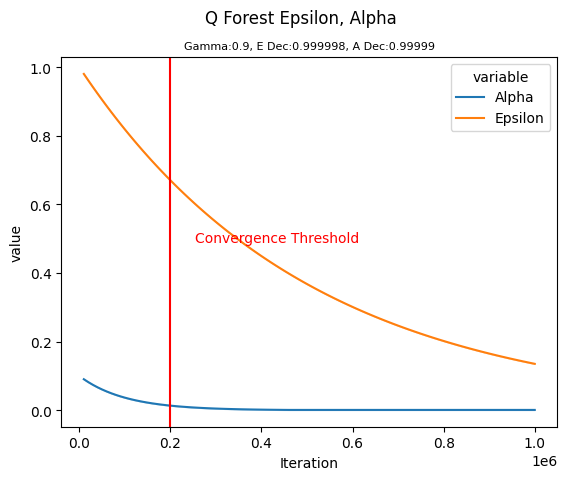
\includegraphics[width=1.2in]{Figures/Q_Forest_Epsilon__Alpha_Gamma_0_9__E_Dec_0_999998__A_Dec_0_99999.png}
  	\end{subfigure}%
	 \begin{subfigure}[b]{0.175\textwidth}
		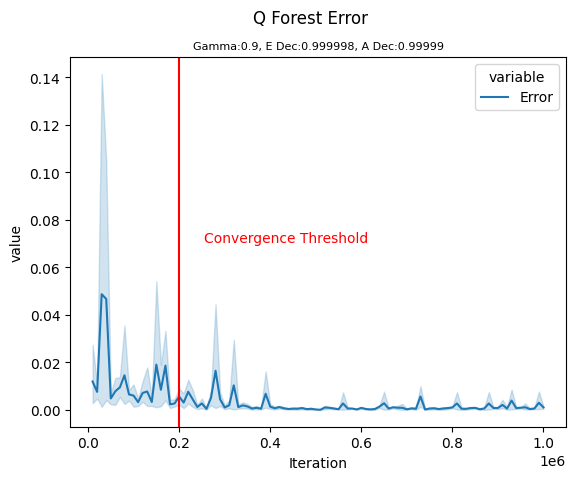
\includegraphics[width=1.2in]{Figures/Q_Forest_Error_Gamma_0_9__E_Dec_0_999998__A_Dec_0_99999.png}
  	\end{subfigure}%
	\begin{subfigure}[b]{0.175\textwidth}
		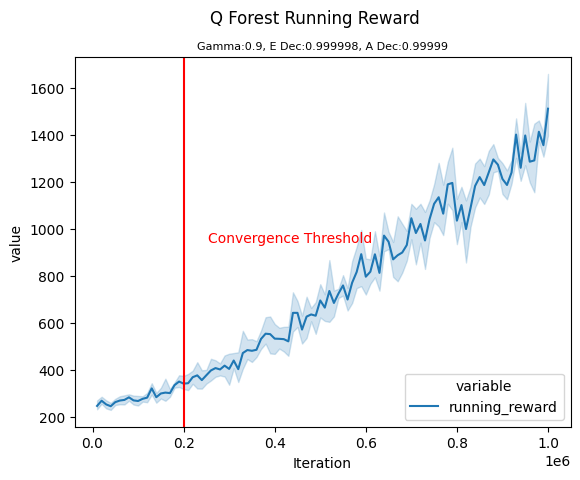
\includegraphics[width=1.2in]{Figures/Q_Forest_Running_Reward_Gamma_0_9__E_Dec_0_999998__A_Dec_0_99999.png}
  	\end{subfigure}
\caption{Forest Q,  $\epsilon$ Decay of .999998, $\alpha$ Decay of 0.99999}
\label{fig:forest_q_e_999998_a_99999_rewards}
\end{figure}

\begin{figure}[!htb]
	\begin{subfigure}[b]{0.25\textwidth}
		\centering
		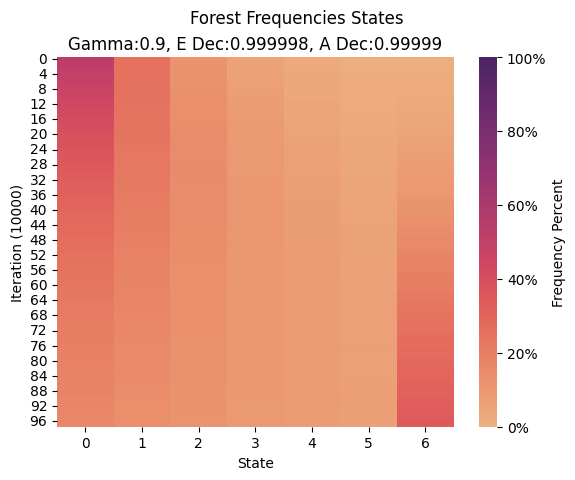
\includegraphics[width=1.75in]{Figures/Forest_Frequencies_States_Gamma_0_9__E_Dec_0_999998__A_Dec_0_99999.png}
  	\end{subfigure}%
	\begin{subfigure}[b]{0.25\textwidth}
		\centering
		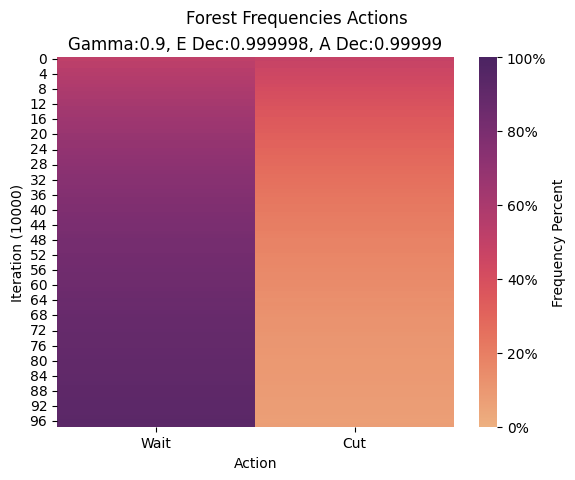
\includegraphics[width=1.75in]{Figures/Forest_Frequencies_Actions_Gamma_0_9__E_Dec_0_999998__A_Dec_0_99999.png}
  	\end{subfigure}%
\caption{Forest Q,  $\epsilon$ Decay of .999998, $\alpha$ Decay of 0.99999}
\label{fig:forest_q_e_999998_a_99999_frequencies}
\end{figure}

\textbf{Figure \ref{fig:forest_q_e_999998_a_99999_rewards}} shows the results of dramatically increasing the decay factor.  The left chart shows that $\epsilon$ remains high throughout the experiment.  Error is more dramatic, but shows the same pattern as before.  The right running reward chart shows the key difference - a strongly rising running reward.  \textbf{Figure \ref{fig:forest_q_e_999998_a_99999_frequencies}} shows the shift from primarily states 0 and 1 to the final state as Q Learning goes on.  Actions also show a strong shift towards waiting with more iterations.  

The key observation is that running reward is still increasing, which is primarily governed by the $\epsilon$ driven exploration.  The action frequency seems to indicate that policy is largely to wait, but exploration is still choosing both actions.  


\begin{figure}[!htb]
	\centering
 	\begin{subfigure}[b]{0.175\textwidth}
		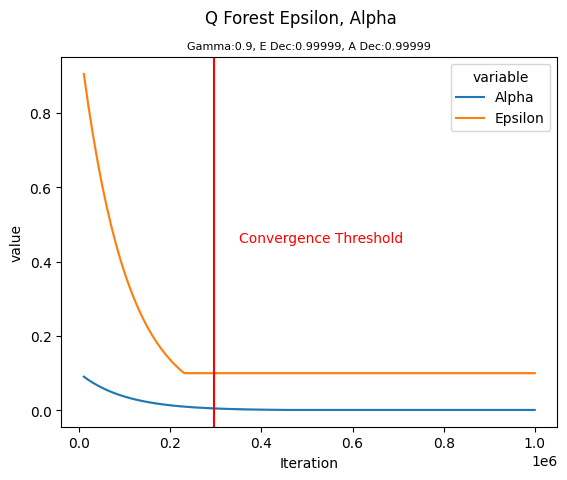
\includegraphics[width=1.2in]{Figures/Q_Forest_Epsilon__Alpha_Gamma_0_9__E_Dec_0_99999__A_Dec_0_99999.png}
  	\end{subfigure}%
	 \begin{subfigure}[b]{0.175\textwidth}
		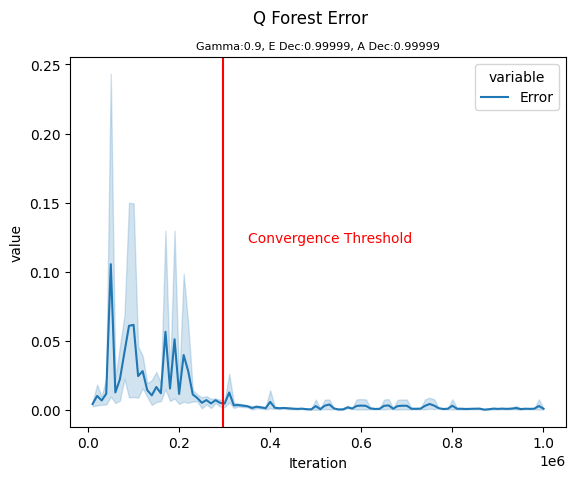
\includegraphics[width=1.2in]{Figures/Q_Forest_Error_Gamma_0_9__E_Dec_0_99999__A_Dec_0_99999.png}
  	\end{subfigure}%
	\begin{subfigure}[b]{0.175\textwidth}
		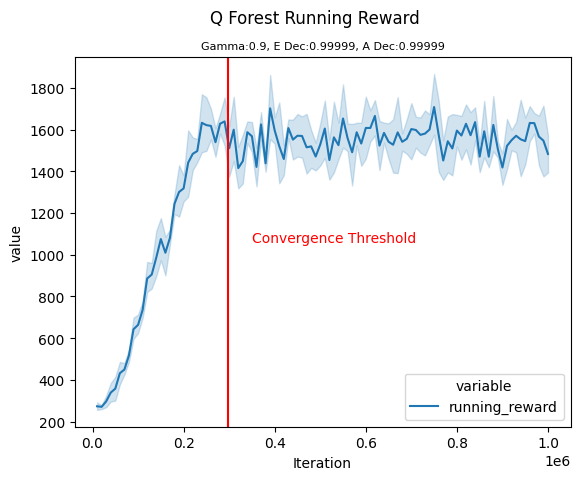
\includegraphics[width=1.2in]{Figures/Q_Forest_Running_Reward_Gamma_0_9__E_Dec_0_99999__A_Dec_0_99999.png}
  	\end{subfigure}
\caption{Forest Q,  $\epsilon$ Decay of .99999, $\alpha$ Decay of 0.99999}
\label{fig:forest_q_e_99999_a_99999_rewards}
\end{figure}

\begin{figure}[!htb]
	\begin{subfigure}[b]{0.25\textwidth}
		\centering
		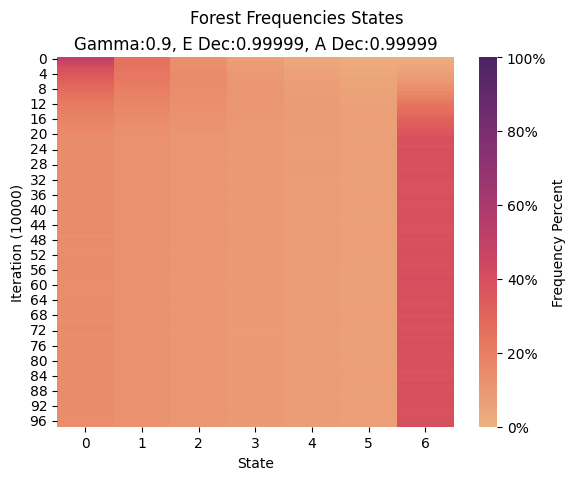
\includegraphics[width=1.75in]{Figures/Forest_Frequencies_States_Gamma_0_9__E_Dec_0_99999__A_Dec_0_99999.png}
  	\end{subfigure}%
	\begin{subfigure}[b]{0.25\textwidth}
		\centering
		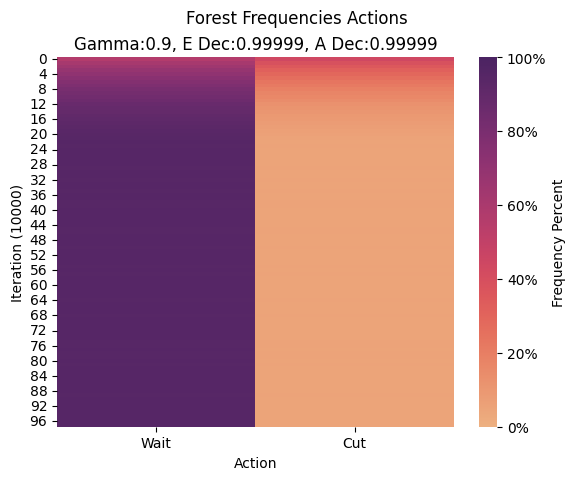
\includegraphics[width=1.75in]{Figures/Forest_Frequencies_Actions_Gamma_0_9__E_Dec_0_99999__A_Dec_0_99999.png}
  	\end{subfigure}%
\caption{Forest Q,  $\epsilon$ Decay of .99999, $\alpha$ Decay of 0.99999}
\label{fig:forest_q_e_99999_a_99999_frequencies}
\end{figure}

\textbf{Figure \ref{fig:forest_q_e_99999_a_99999_rewards}} shows a good overall solution for Forest.  We see $\epsilon$ and $\alpha$ declining over about 300,000 iterations.  Error declines as well.  The running reward chart is key, showing us reaching a very value quickly, reaching a solved plateau.   \textbf{Figure \ref{fig:forest_q_e_99999_a_99999_frequencies}} frequency charts in line with the reward charts.  

After looking at the different runs and output, I chose running reward as the convergence criteria, creating a threshold for when the running reward stops increasing.  I used large windows and averages to prevent the noise from triggering the threshold.  I didn't move this convergence threshold back into the MDP toolbox, but it would be possible to do this.  The running reward chart serves as the convergence chart for Q Learning.

\subsection{Lake MDP} 
I was optimistic that \textbf{\emph{Lake MDP}} would be an easy extension of Forest, but the first key issue was that Lake is an episodic MDP.  Looking at the data, the state frequencies where all in holes and the goal state.  This was partially a function of removing the random reset of state every 100 episodes, which would have glossed over the underlying challenge.  The challenge was that the transition model from Frozen Lake was that the next transitions from a hole or goal was back to itself.  The MDP implementation did not have a concept of terminal states.  One change I could have made was to change those transition states back to the start, but there would not be a concept of episode.  Instead, I created a modified episodic Q learning that takes a list of terminal states and tracks episodes.  For Lake Q Learning, I used episodes instead of iterations for charting, which I thought was a better representation for episodic learning, although it makes comparisons between Lake and Forest are a bit tricky.

With the episodic changes, the Small and Medium Lake maps were solved using  $\epsilon$ and $\alpha$ decays from Forest.  With the Large Lake map, I was not producing any useful convergence.  I moved up to 100 billion iterations and extremely large $\epsilon$ and $\alpha$ decays, with no progress.  Looking at the frequency charts, all visitation was close to the start.   \textbf{Figure \ref{fig:forest_q_reachability}} showed the challenge of reaching end states in the Forest MDP.  After consideration, with the highly stochastic actions and holes ending episodes, while I couldn't calculate it, the chance of reaching the end state without random restarts was effectively zero.  Ouch!

Based on this, I reduced the Large map size to 16 X 16.  I was still not able to solve, so I started to remove holes until I started to get traction and used this map. I went back and reran VI and PI using this as the new baseline Large Lake Map  (\emph{which is what is used through out the report now}).  





\begin{figure}[!htb]
	\centering
 	\begin{subfigure}[b]{0.175\textwidth}
		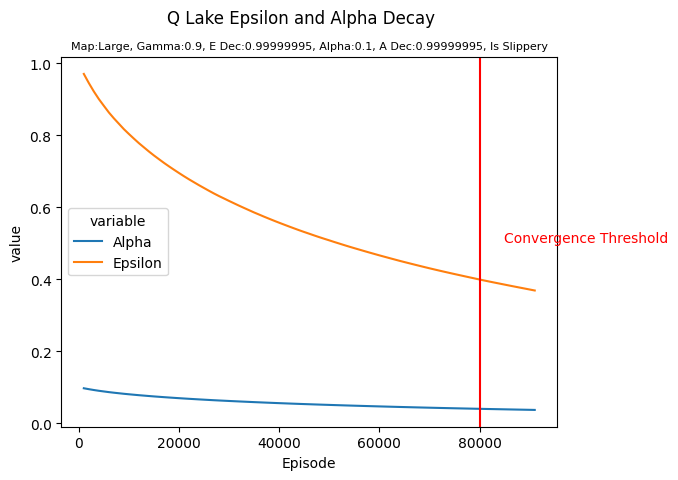
\includegraphics[width=1.2in]{Figures/Q_Lake_Epsilon_and_Alpha_Decay_Map_Large__Gamma_0_9__E_Dec_0_99999995__Alpha_0_1__A_Dec_0_99999995__Is_Slippery.png}
  	\end{subfigure}%
	 \begin{subfigure}[b]{0.175\textwidth}
		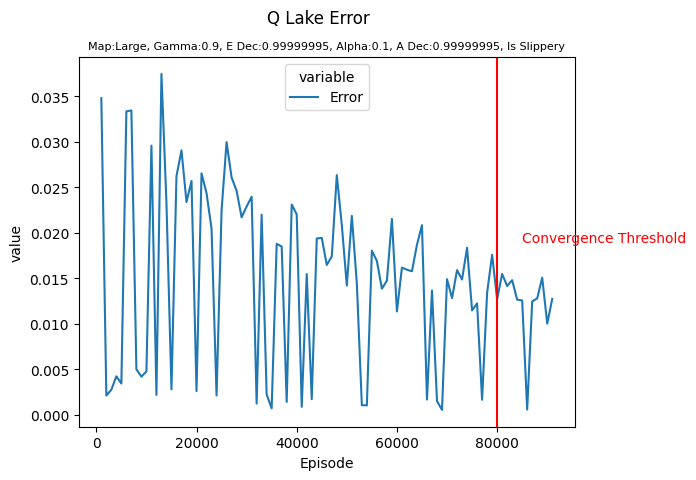
\includegraphics[width=1.2in]{Figures/Q_Lake_Error_Map_Large__Gamma_0_9__E_Dec_0_99999995__Alpha_0_1__A_Dec_0_99999995__Is_Slippery.png}
  	\end{subfigure}%
	\begin{subfigure}[b]{0.175\textwidth}
		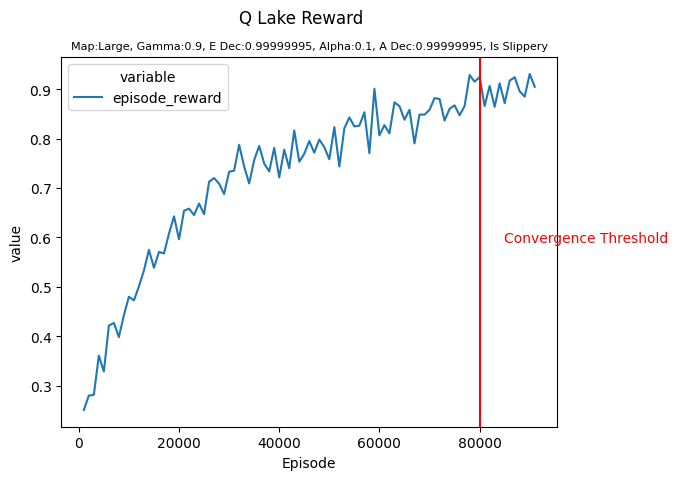
\includegraphics[width=1.2in]{Figures/Q_Lake_Reward_Map_Large__Gamma_0_9__E_Dec_0_99999995__Alpha_0_1__A_Dec_0_99999995__Is_Slippery.png}
  	\end{subfigure}
\caption{Lake Q,  $\epsilon$ Decay of 0.99999995, $\alpha$ Decay of 0.99999995}
\label{fig:lake_q_e_99999995_a_99999995_rewards}
\end{figure}

\begin{figure}[!htb]
	\begin{subfigure}[b]{0.25\textwidth}
		\centering
		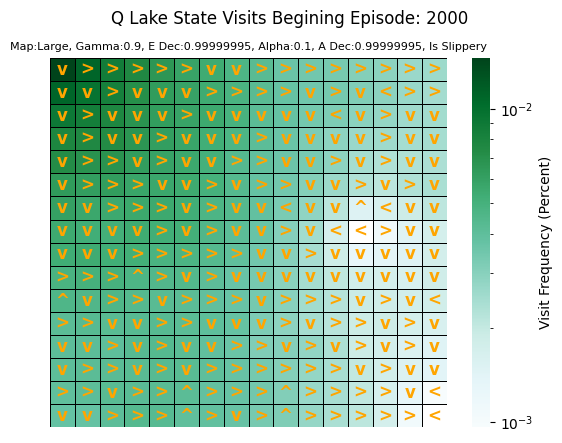
\includegraphics[width=1.75in]{Figures/Q_Lake_State_Visits_Begining_Episode__2000_Map_Large__Gamma_0_9__E_Dec_0_99999995__Alpha_0_1__A_Dec_0_99999995__Is_Slippery.png}
		\caption{Initial Episodes}
  	\end{subfigure}%
	\begin{subfigure}[b]{0.25\textwidth}
		\centering
		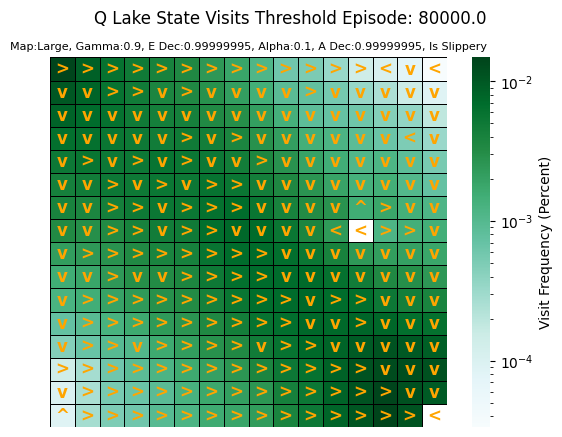
\includegraphics[width=1.75in]{Figures/Q_Lake_State_Visits_Threshold_Episode__80000_0_Map_Large__Gamma_0_9__E_Dec_0_99999995__Alpha_0_1__A_Dec_0_99999995__Is_Slippery.png}
		\caption{Threshold Episodes}
  	\end{subfigure}%
\caption{Lake Q,  $\epsilon$ Decay of 0.99999995, $\alpha$ Decay of 0.99999995}
\label{fig:lake_q_e_99999995_a_99999995_maps}
\end{figure}


\begin{figure}[!htb]
	\centering
 	\begin{subfigure}[b]{0.175\textwidth}
		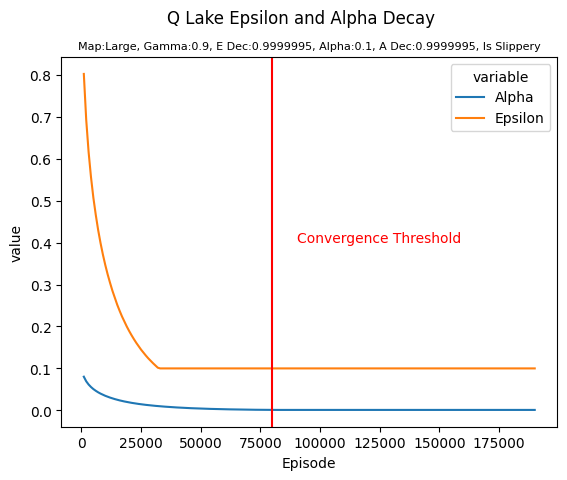
\includegraphics[width=1.2in]{Figures/Q_Lake_Epsilon_and_Alpha_Decay_Map_Large__Gamma_0_9__E_Dec_0_9999995__Alpha_0_1__A_Dec_0_9999995__Is_Slippery.png}
  	\end{subfigure}%
	 \begin{subfigure}[b]{0.175\textwidth}
		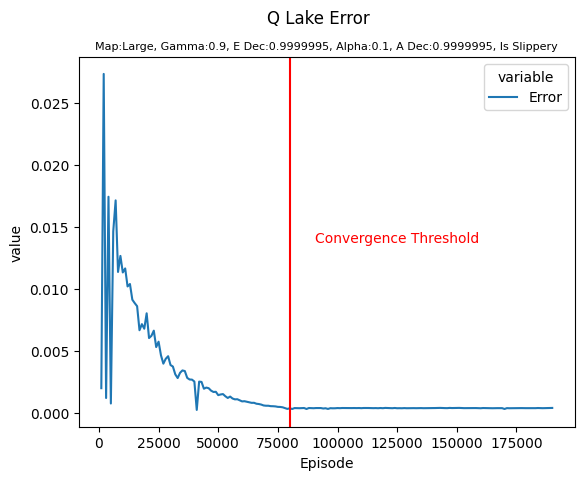
\includegraphics[width=1.2in]{Figures/Q_Lake_Error_Map_Large__Gamma_0_9__E_Dec_0_9999995__Alpha_0_1__A_Dec_0_9999995__Is_Slippery.png}
  	\end{subfigure}%
	\begin{subfigure}[b]{0.175\textwidth}
		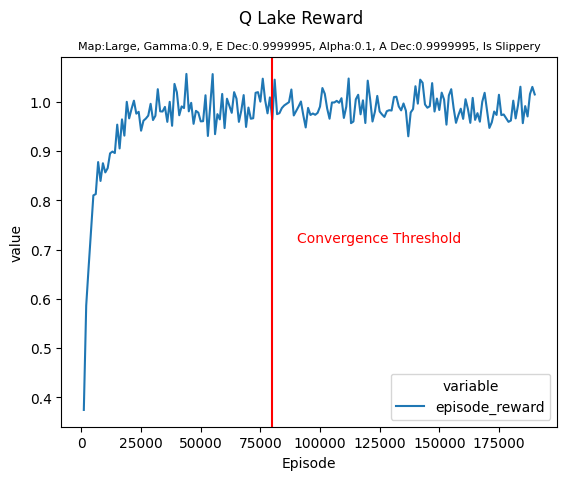
\includegraphics[width=1.2in]{Figures/Q_Lake_Reward_Map_Large__Gamma_0_9__E_Dec_0_9999995__Alpha_0_1__A_Dec_0_9999995__Is_Slippery.png}
  	\end{subfigure}
\caption{Lake Q,  $\epsilon$ Decay of 0.9999995, $\alpha$ Decay of 0.9999995}
\label{fig:lake_q_e_9999995_a_9999995_rewards}
\end{figure}

\begin{figure}[!htb]
	\begin{subfigure}[b]{0.25\textwidth}
		\centering
		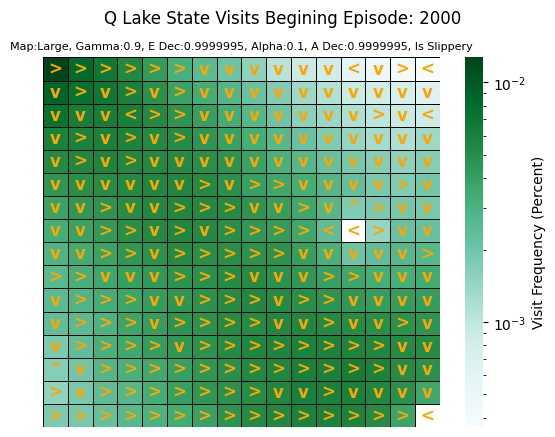
\includegraphics[width=1.75in]{Figures/Q_Lake_State_Visits_Begining_Episode__2000_Map_Large__Gamma_0_9__E_Dec_0_9999995__Alpha_0_1__A_Dec_0_9999995__Is_Slippery.png}
		\caption{Initial Episodes}
  	\end{subfigure}%
	\begin{subfigure}[b]{0.25\textwidth}
		\centering
		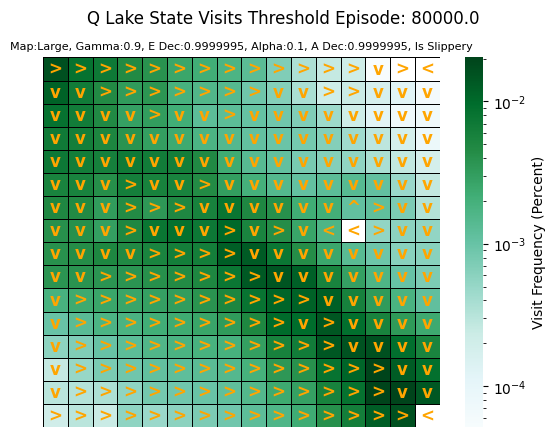
\includegraphics[width=1.75in]{Figures/Q_Lake_State_Visits_Threshold_Episode__80000_0_Map_Large__Gamma_0_9__E_Dec_0_9999995__Alpha_0_1__A_Dec_0_9999995__Is_Slippery.png}
		\caption{Threshold Episodes}
  	\end{subfigure}%
\caption{Lake Q,  $\epsilon$ Decay of 0.9999995, $\alpha$ Decay of 0.9999995}
\label{fig:lake_q_e_9999995_a_9999995_maps}
\end{figure}




Initial Alpha value can also be larger.  Exploration with this showed some advantages, but the final model presented was best.



\section{Summary}
Tuning needed
PI - none
VI - estop
Q Learning - epsilon, epsilon decay, alpha, alpha decay
A lot of interplay between them and environment
easy to fall into local minima
very easy to miss key rewards

No floor on epsilon \ alpha

Policy far from the reward \ goal state can be very different depending on e stop (VI) and a bunch of things in Q Learning


Left 
\section{References}
\begin{tabular}{l p{2.75in}}
\\
1 & Markov Decision Processes (MDP) Toolbox, https://miat.inrae.fr/MDPtoolbox/ Accessed: 11/1/2022.
\\
2 & Markov Decision Process (MDP) Toolbox for Python, https://github.com/sawcordwell/pymdptoolbox: Accessed: 11/1/2022.
\\
3 & hiive Fork: Markov Decision Process (MDP) Toolbox for Python, https://github.com/hiive/hiivemdptoolbox: Accessed: 11/1/2022.
\\
4 & Brockman, G. et al., 2016. Openai gym.
\\
5 & Openai gym Frozen Lake Documentation,  https://www.gymlibrary.dev/environments/toy\_text/frozen\_lake/: Accessed: 11/1/2022.

\end{tabular}
\end{document}
